\documentclass[letterpaper,12pt,fleqn]{article}
\usepackage{matharticle}
\pagestyle{empty}
\begin{document}
\section*{Introduction}

A brief history of functional analysis:

\begin{tabular}{cll}
  1900 & Ivar Fredholm & Paper on integral equations \\
  \\
  & & \parbox{3in}{Given kernel $K(x,y)$, find $F$ for: \\
    $\int_a^bK(x,y)F(y)dy=g(x)$ or \\
    $F(x)-\int_a^bK(x,y)F(y)dy=g(x)$} \\
  \\
  1902 & Henri Lebesque & Thesis on measure theory and integration \\
  \\
  1906 & David Hilbert & Paper on spectral theory \\
  \\
  1906 & Maurice Ren\'{e} Fr\'{e}chet & Thesis on metric spaces \\
  \\
  1910-1 & Marcel Riesz & Paper on $C[a,b]$ and $L^p[a,b]$ \\
  \\
  1922 & Stefan Banach & Thesis on normed spaces \\
  \\
  1928 & Fr\'{e}chet & Book on abstract spaces \\
  \\
  1932 & Banach & Book on linear operators
\end{tabular}

\vspace {0.5in}

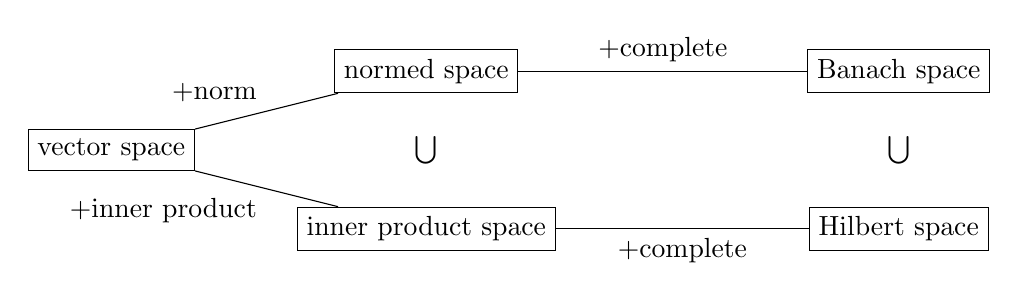
\begin{tikzpicture}
  \node [draw] (VS) at (0,0) {vector space};
  \node [draw] (NS) at (4,1) {normed space};
  \node [draw] (IPS) at (4,-1) {inner product space};
  \node [draw] (BS) at (10,1) {Banach space};
  \node [draw] (HS) at (10,-1) {Hilbert space};
  \draw (VS) -- node [above left] {+norm} (NS);
  \draw (VS) -- node [below left] {+inner product} (IPS);
  \draw (NS) -- node [above] {+complete} (BS);
  \draw (IPS) -- node [below] {+complete} (HS);
  \node at (4,0) {$\bigcup$};
  \node at (10,0) {$\bigcup$};
\end{tikzpicture}

\end{document}
